
\section{Programming Yosys Extensions}

\begin{frame}
\sectionpage
\end{frame}

%%%%%%%%%%%%%%%%%%%%%%%%%%%%%%%%%%%%%%%%%%%%%%%%%%%%%%%%%%%%%%%%%%%%%%%%%%%%%

\subsection{Program Components and Data Formats}

\begin{frame}{\subsecname}
\begin{center}
\begin{tikzpicture}[scale=0.6, every node/.style={transform shape}]
	\tikzstyle{process} = [draw, fill=green!10, rectangle, minimum height=3em, minimum width=10em, node distance=15em]
	\tikzstyle{data} = [draw, fill=blue!10, ellipse, minimum height=3em, minimum width=7em, node distance=15em]
	\node[process] (vlog) {Verilog Frontend};
	\node[process, dashed, fill=green!5] (vhdl) [right of=vlog] {VHDL Frontend};
	\node[process] (ilang) [right of=vhdl] {Other Frontends};
	\node[data] (ast) [below of=vlog, node distance=5em, xshift=7.5em] {AST};
	\node[process] (astfe) [below of=ast, node distance=5em] {AST Frontend};
	\node[data] (rtlil) [below of=astfe, node distance=5em, xshift=7.5em] {RTLIL};
	\node[process] (pass) [right of=rtlil, node distance=5em, xshift=7.5em] {Passes};
	\node[process] (vlbe) [below of=rtlil, node distance=7em, xshift=-13em] {Verilog Backend};
	\node[process] (ilangbe) [below of=rtlil, node distance=7em, xshift=0em] {ILANG Backend};
	\node[process, fill=green!5] (otherbe) [below of=rtlil, node distance=7em, xshift=+13em] {Other Backends};

	\draw[-latex] (vlog) -- (ast);
	\draw[-latex] (vhdl) -- (ast);
	\draw[-latex] (ast) -- (astfe);
	\draw[-latex] (astfe) -- (rtlil);
	\draw[-latex] (ilang) -- (rtlil);
	\draw[latex-latex] (rtlil) -- (pass);
	\draw[-latex] (rtlil) -- (vlbe);
	\draw[-latex] (rtlil) -- (ilangbe);
	\draw[-latex] (rtlil) -- (otherbe);
\end{tikzpicture}
\end{center}
\end{frame}

%%%%%%%%%%%%%%%%%%%%%%%%%%%%%%%%%%%%%%%%%%%%%%%%%%%%%%%%%%%%%%%%%%%%%%%%%%%%%

\subsection{Simplified RTLIL Entity-Relationship Diagram}

\begin{frame}{\subsecname}
Between passses and frontends/backends the design in stored in Yosys' internal RTLIL (RTL Intermediate Language) format. For
writing Yosys extensions it is key to understand this format.

\bigskip
\begin{center}
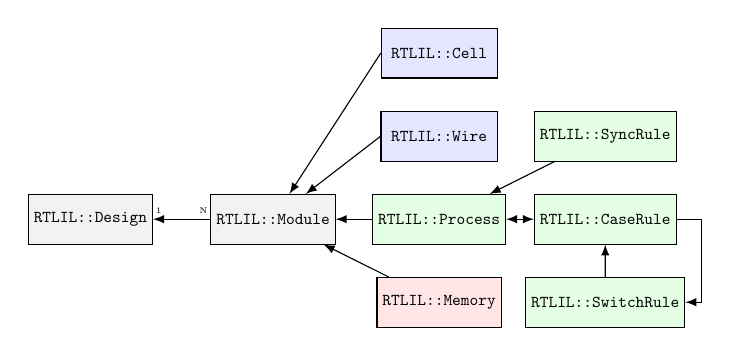
\begin{tikzpicture}[scale=0.6, every node/.style={transform shape}]
	\tikzstyle{entity} = [draw, fill=gray!10, rectangle, minimum height=3em, minimum width=7em, node distance=5em, font={\ttfamily}]
	\node[entity] (design) {RTLIL::Design};
	\node[entity] (module) [right of=design, node distance=11em] {RTLIL::Module} edge [-latex] node[above] {\tiny 1 \hskip3em N} (design);

	\node[entity] (process) [fill=green!10, right of=module, node distance=10em] {RTLIL::Process} (process.west) edge [-latex] (module);
	\node[entity] (memory) [fill=red!10, below of=process] {RTLIL::Memory} edge [-latex] (module);
	\node[entity] (wire) [fill=blue!10, above of=process] {RTLIL::Wire} (wire.west) edge [-latex] (module);
	\node[entity] (cell) [fill=blue!10, above of=wire] {RTLIL::Cell} (cell.west) edge [-latex] (module);

	\node[entity] (case) [fill=green!10, right of=process, node distance=10em] {RTLIL::CaseRule} edge [latex-latex] (process);
	\node[entity] (sync) [fill=green!10, above of=case] {RTLIL::SyncRule} edge [-latex] (process);
	\node[entity] (switch) [fill=green!10, below of=case] {RTLIL::SwitchRule} edge [-latex] (case);
	\draw[latex-] (switch.east) -- ++(1em,0) |- (case.east);
\end{tikzpicture}
\end{center}
\end{frame}

%%%%%%%%%%%%%%%%%%%%%%%%%%%%%%%%%%%%%%%%%%%%%%%%%%%%%%%%%%%%%%%%%%%%%

\subsection{RTLIL without memories and processes}

\begin{frame}[fragile]{\subsecname}
After the command {\tt proc} and {\tt memory} (or {\tt memory -nomap}), we are left with a much simpler version of RTLIL:

\begin{center}
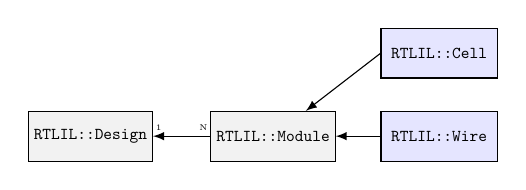
\begin{tikzpicture}[scale=0.6, every node/.style={transform shape}]
	\tikzstyle{entity} = [draw, fill=gray!10, rectangle, minimum height=3em, minimum width=7em, node distance=5em, font={\ttfamily}]
	\node[entity] (design) {RTLIL::Design};
	\node[entity] (module) [right of=design, node distance=11em] {RTLIL::Module} edge [-latex] node[above] {\tiny 1 \hskip3em N} (design);

	\node[entity] (wire) [fill=blue!10, right of=module, node distance=10em] {RTLIL::Wire} (wire.west) edge [-latex] (module);
	\node[entity] (cell) [fill=blue!10, above of=wire] {RTLIL::Cell} (cell.west) edge [-latex] (module);
\end{tikzpicture}
\end{center}

\bigskip
Many command simply choose to only work on this simpler version:
\begin{lstlisting}[xleftmargin=0.5cm, basicstyle=\ttfamily\fontsize{8pt}{10pt}\selectfont]
if (module->processes.size() != 0 || module->memories.size() != 0)
    log_error("This command does not operate on modules with processes "
              "and/or memories! Run 'proc' and 'memory' first.\n");
\end{lstlisting}

\bigskip
So we only discuss this version of RTLIL in this presentation.
\end{frame}

